\section{Legacy Results, Diagnostics, and Provenance}
\label{app:legacy}

This appendix records the material retained from the earlier draft.  The
current buffered analysis is authoritative: an older statement is carried
forward only when it is unchanged, follows under the assumptions used here, or
is explicitly marked as a result for a different observation model.
Table~\ref{tab:legacy-theory-map} makes that relationship explicit.

\begin{table}[t]
\centering
\small
\begin{tabular}{p{0.24\linewidth}p{0.31\linewidth}p{0.36\linewidth}}
\toprule
Earlier result & Status in this paper & Reason \\
\midrule
Correct-region polytope and MILP &
Retained in Section~\ref{sec:method-margin} and
Eq.~(\ref{eq:buffered-milp}) &
The geometry is unchanged; the MILP threshold is shifted by the calibrated
buffer and its numerical strictness tolerance is now explicit. \\
Uniform convergence over questions &
Retained as the slow-\(Q\) component of Theorem~\ref{thm:buffered-main} &
The hyperplane-arrangement argument gives complexity
\((K-1)\log(eAQ)\), without requiring a margin condition. \\
Accelerated \(Q\)-rate &
Replaced by Theorem~\ref{thm:fast} &
A margin condition alone is insufficient.  Fast learning additionally needs
absolute boundary control and identifiable risk growth. \\
Finite-generation \(N\)-term &
Retained and strengthened by buffering &
The buffer pays boundary mass only at the fixed comparator rather than
requiring a uniform margin condition at a random learned weight. \\
Joint \((N,Q)\) rate &
Replaced by Theorem~\ref{thm:buffered-main}, with an optional fast version in
Theorem~\ref{thm:fast} &
The robust default is \(Q^{-1/2}+N^{-\beta/2}\); a faster \(Q\)-term is
conditional on geometric identifiability. \\
Rollout minimax lower bound &
Retained below as a complementary observation-model result &
It concerns prediction from sampled answers with the gold answer hidden, not
the supervised weight-learning experiment of the main theorem. \\
Compute-allocation corollaries &
Not asserted as results of the buffered-only paper &
They depend on a chosen cost model and rate constants.  The old formulas
remain preserved in the untouched source draft, but are not needed for the
estimator or its guarantee. \\
\bottomrule
\end{tabular}
\caption{Disposition of the principal results from the earlier draft.  No
unsupported fast-\(Q\) claim is silently inherited.}
\label{tab:legacy-theory-map}
\end{table}

\subsection{Supporting finite-generation facts}
\label{app:legacy-support}

The first fact explains why taking the hardest wrong answer changes constants
but not the concentration scale.

\begin{lemma}[Stability of the minimum]
\label{lem:legacy-min-stability}
For finite vectors \(x=(x_a)_{a\in I}\) and \(y=(y_a)_{a\in I}\),
\[
\left|\min_{a\in I}x_a-\min_{a\in I}y_a\right|
\le \max_{a\in I}|x_a-y_a|.
\]
Consequently, for every problem \(q\) and \(w\in\Delta_K\),
\[
|\widehat M_q(w)-M_q(w)|
\le
\max_{a\ne a^\star(q)}
\left|\left\langle
w,\widehat\Delta_{q,a}-\Delta_{q,a}
\right\rangle\right|.
\]
\end{lemma}

\begin{proof}
Let \(a_x\) and \(a_y\) minimize \(x\) and \(y\), respectively.  Then
\(\min x-\min y=x_{a_x}-y_{a_y}\le x_{a_y}-y_{a_y}\le
\max_a|x_a-y_a|\).  Interchanging \(x\) and \(y\) gives the reverse
inequality.  The margin statement follows by substitution.
\end{proof}

\begin{lemma}[Fixed-weight sign reliability]
\label{lem:legacy-sign}
Assume independent generations across models and draws.  For fixed \(q,w\), let
\(m=|M_q(w)|>0\).  There is a universal \(c>0\) such that
\[
\mathbb P_{\rm gen}\!\left(
\mathbf 1\{\widehat M_q(w)\le0\}\ne
\mathbf 1\{M_q(w)\le0\}\mid q
\right)
\le
2(A-1)\exp\!\left(
-\frac{cNm^2}{\|w\|_2^2}
\right).
\]
In particular, the right side is at most
\(2(A-1)e^{-cNm^2}\) for \(w\in\Delta_K\).
\end{lemma}

\begin{proof}
For a fixed wrong answer \(a\), the empirical score-gap error is a weighted
sum of \(KN\) independent, centered, bounded variables.  Hoeffding's lemma
makes it sub-Gaussian with variance proxy \(C\|w\|_2^2/N\).  A sign change of
the minimum requires at least one contender gap to move by \(m\); apply the
sub-Gaussian tail bound and union bound over at most \(A-1\) contenders.
\end{proof}

The next counterexample is about the raw plug-in risk, not buffered ERM.  It
shows why a punctured condition that ignores mass exactly at zero cannot by
itself guarantee convergence of raw empirical signs.

\begin{proposition}[Zero-margin atom for raw plug-in risk]
\label{prop:legacy-zero-atom}
There is a one-model, two-answer instance satisfying
\(\mathbb P(0<|M_q(w^\star)|\le t)=0\) for every \(t>0\), while for every odd
\(N\),
\[
|R_N(w^\star)-R(w^\star)|=\frac12.
\]
\end{proposition}

\begin{proof}
Let the gold and wrong answers each have probability \(1/2\).  Then
\(M_q(w^\star)=0\), and ties count as errors, so \(R(w^\star)=1\).  If
\(Z\sim{\rm Binomial}(N,1/2)\), the empirical margin for odd \(N\) is
\((2Z-N)/N\), which is negative with probability \(1/2\).  Hence
\(R_N(w^\star)=1/2\).  Theorem~\ref{thm:buffered-main} does not make this
mistake: its one-sided comparator condition charges only the additional
positive-margin band created by the buffer.
\end{proof}

\begin{theorem}[Recovery of exact-output aggregation]
\label{thm:legacy-exact-limit}
Fix \(w\in\Delta_K\) and suppose
\(\mathbb P_q\{M_q(w)=0\}=0\).  If every empirical answer frequency is formed
from \(N\) independent generations, then
\[
\lim_{N\to\infty}
\mathbb P_{q,\rm gen}\{\widehat M_q^{(N)}(w)\le0\}
=
\mathbb P_q\{M_q(w)\le0\}.
\]
\end{theorem}

\begin{proof}
For fixed \(q\), the strong law and finiteness of the model and answer sets
give uniform coordinate convergence of empirical answer probabilities.
Lemma~\ref{lem:legacy-min-stability} then gives
\(\widehat M_q^{(N)}(w)\to M_q(w)\) almost surely.  The error indicator
converges away from zero, and the no-boundary-mass assumption plus dominated
convergence completes the proof.
\end{proof}

\begin{corollary}[Separated-margin finite-generation term]
\label{cor:legacy-separated}
If \(|M_q(w^\star)|\ge\gamma>0\) almost surely, then
\[
|R_N(w^\star)-R(w^\star)|
\le 2(A-1)e^{-cN\gamma^2}.
\]
\end{corollary}

\begin{proof}
Integrate Lemma~\ref{lem:legacy-sign} over \(q\) and use
\(\|w^\star\|_2\le1\).
\end{proof}

\subsection{A complementary rollout lower bound}
\label{app:legacy-lower-bound}

The supervised problem in the main text learns \(w\) from labeled questions.
The following retained theorem addresses a different prediction-time model:
the rule sees only \(N\) sampled binary answers and does not observe the gold
answer or an identifying problem feature.  Stating that distinction is
essential; the result is evidence that finite-generation ambiguity can be
information-theoretic, not a lower bound for every supervised protocol.

\begin{theorem}[Rollout-only minimax lower bound]
\label{thm:legacy-rollout-lower}
For \(\beta\ge0\) and \(C_m\ge1\), let
\(\mathfrak D_\beta(C_m)\) be the binary one-model distributions satisfying
\(\mathbb P(0<M_q\le t)\le C_m t^\beta\).  Under the rollout-only observation
model above, there is \(c_{\beta,C_m}>0\) such that
\[
\inf_{\psi_N}\sup_{\mathcal D\in\mathfrak D_\beta(C_m)}
\left\{
R_N^{\psi}(\mathcal D)-R_\infty^\star(\mathcal D)
\right\}
\ge c_{\beta,C_m}N^{-\beta/2}.
\]
\end{theorem}

\begin{proof}
Set \(\gamma_N=1/(8\sqrt N)\) and place mass
\(\alpha_N=c_\alpha\gamma_N^\beta\) on near-tie problems, where
\(c_\alpha=\min\{C_m/2,1/2\}\).  Conditional on the hidden gold bit, sampled
answers follow Bernoulli laws with means \((1+\gamma_N)/2\) and
\((1-\gamma_N)/2\).  Their \(N\)-fold KL divergence is bounded by a universal
constant, so Le Cam's two-point bound gives testing error at least \(3/8\).
The infinite-rollout oracle is correct, while every finite rule incurs at
least \((3/8)\alpha_N\), which is the displayed order.  The remaining mass can
be placed on deterministic easy problems, and the construction satisfies the
stated margin condition.
\end{proof}

\subsection{Legacy mechanism checks}
\label{app:legacy-synthetic}

Table~\ref{tab:legacy-synthetic} preserves the two small simulations reported
in the earlier note.  They are useful mechanism checks, but the original
per-replicate artifacts are unavailable; the numbers are therefore reported as
legacy values rather than a fresh rerun.  The first four columns show that
sign errors concentrate in the \(N^{-1/2}\) boundary band.  The last column
reports optimization bias at fixed \(Q=60\).

\begin{table}[t]
\centering
\small
\begin{tabular}{rcccc}
\toprule
\(N\) & band mass & in-band flip & out-of-band flip &
in-sample minus true accuracy \\
\midrule
20   & 0.465 & 0.189 & 0.004 & 0.054 \\
80   & 0.252 & 0.175 & 0.002 & 0.029 \\
320  & 0.119 & 0.198 & 0.001 & 0.018 \\
1280 & 0.060 & 0.192 & 0.000 & 0.013 \\
\bottomrule
\end{tabular}
\caption{Legacy synthetic mechanism checks.  Band mass is
\(\mathbb P(|M_q|\le N^{-1/2})\); flip columns condition on being inside or
outside that band.  The final column is the earlier winner-selection diagnostic
at fixed \(Q=60\).}
\label{tab:legacy-synthetic}
\end{table}

\subsection{Reproducible benchmark context}
\label{app:legacy-real}

We also retain a reproducible legacy analysis over tracked generation JSONL
files.  It compares the original MILP with a bootstrap-stability plus
max-margin variant; it does \emph{not} evaluate the statistically calibrated
buffer \(\varepsilon_N\) of Theorem~\ref{thm:buffered-main}.  Accordingly,
Table~\ref{tab:legacy-real} is context for the empirical motivation, not direct
validation of the new estimator.

\begin{table}[t]
\centering
\small
\begin{tabular}{lrrrr}
\toprule
Benchmark & \(Q\) & \(K\) & vanilla gap & stability+margin gap \\
\midrule
AIME 2024    & 30  & 11 & 0.0951 & 0.0946 \\
AIME 2025    & 30  & 11 & 0.1523 & 0.1279 \\
GPQA-Diamond & 198 & 6  & 0.0683 & 0.0494 \\
MATH-500     & 500 & 7  & 0.0167 & 0.0150 \\
\bottomrule
\end{tabular}
\caption{Absolute train--test gaps from the reproducible legacy JSONL
analysis.  Averaged over benchmarks, the gap falls from \(0.0831\) to
\(0.0717\), a \(13.67\%\) closure.}
\label{tab:legacy-real}
\end{table}

The same run reports \(26.00\%\) mean gap closure across the five stored
cross-benchmark directions.  These aggregate values are descriptive because
the benchmark sizes, model sets, and train fractions differ.

\begin{table}[t]
\centering
\small
\begin{tabular}{lrrr}
\toprule
Benchmark & \(Q\) & empirical risk & uniform-prior bound \\
\midrule
AIME 2024    & 30  & 0.000 & 2.216 \\
AIME 2025    & 30  & 0.200 & 2.277 \\
GPQA-Diamond & 198 & 0.250 & 0.541 \\
MATH-500     & 500 & 0.023 & 0.369 \\
\bottomrule
\end{tabular}
\caption{Retained PAC--Bayes diagnostic from the same run.  The AIME bounds
are vacuous; the table is not used in any theorem.}
\label{tab:legacy-pacbayes}
\end{table}

\begin{figure}[t]
\centering
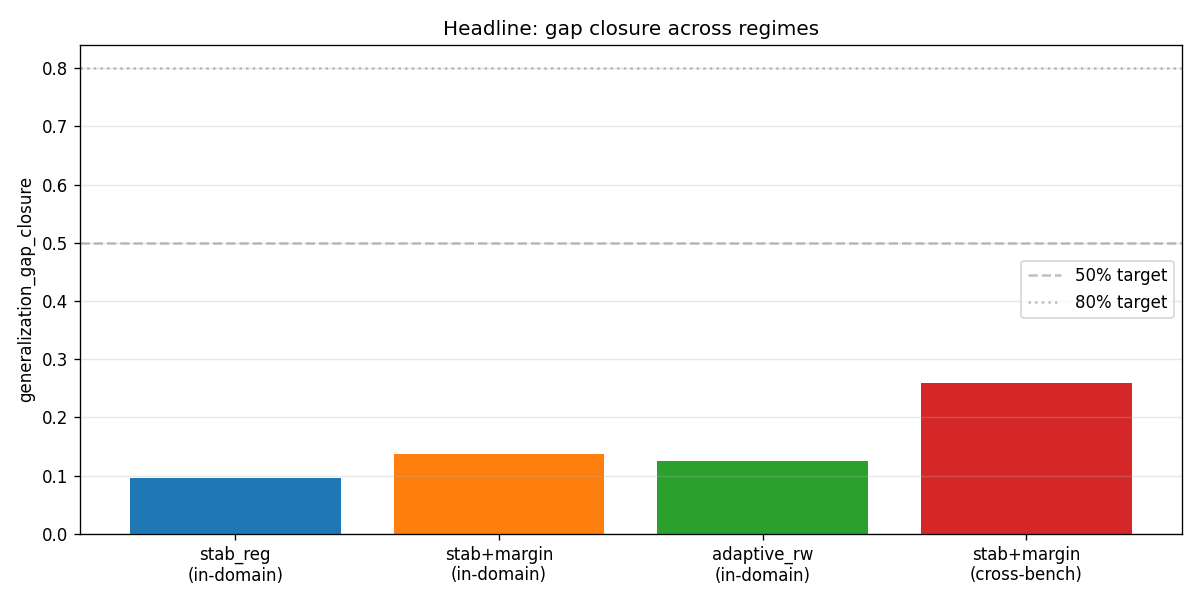
\includegraphics[width=0.49\linewidth]{buffered_figures/legacy_gap_closure.png}
\hfill
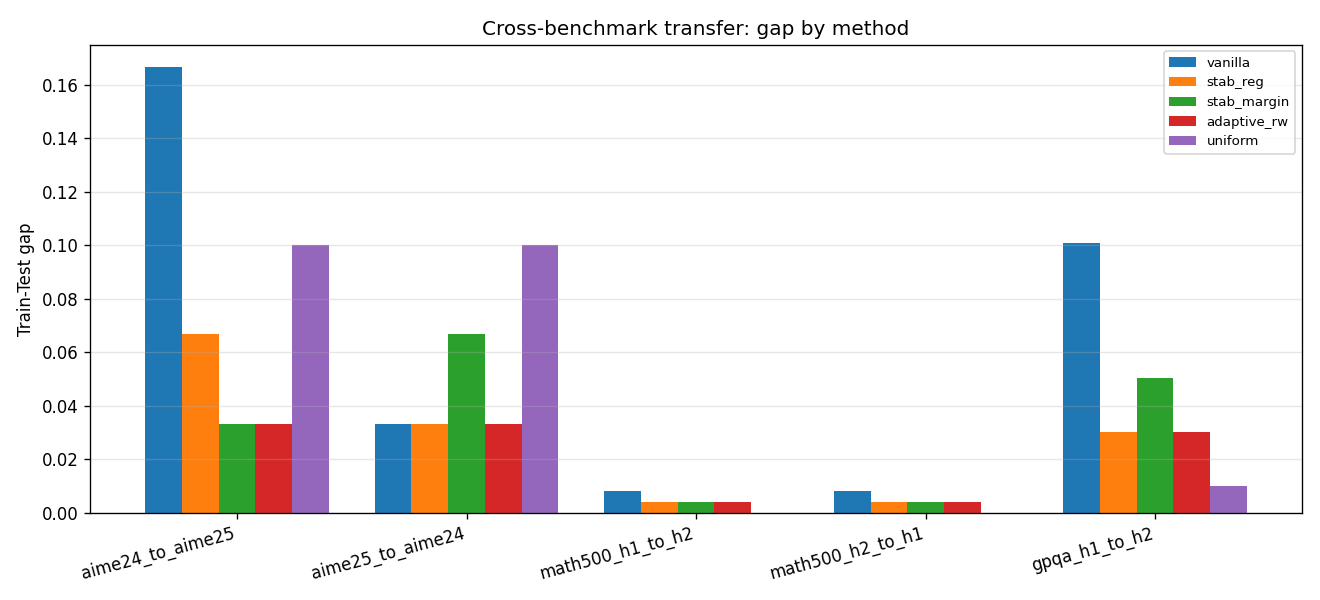
\includegraphics[width=0.49\linewidth]{buffered_figures/legacy_cross_benchmark.png}
\caption{Reproducible legacy diagnostics.  Left: in-domain gap closure.
Right: cross-benchmark train--test gaps.  Both figures are regenerated from
the tracked JSONL files by \texttt{zhi\_code/src/pacbayes\_boinf.py}.}
\label{fig:legacy-gap}
\end{figure}

\begin{figure}[t]
\centering
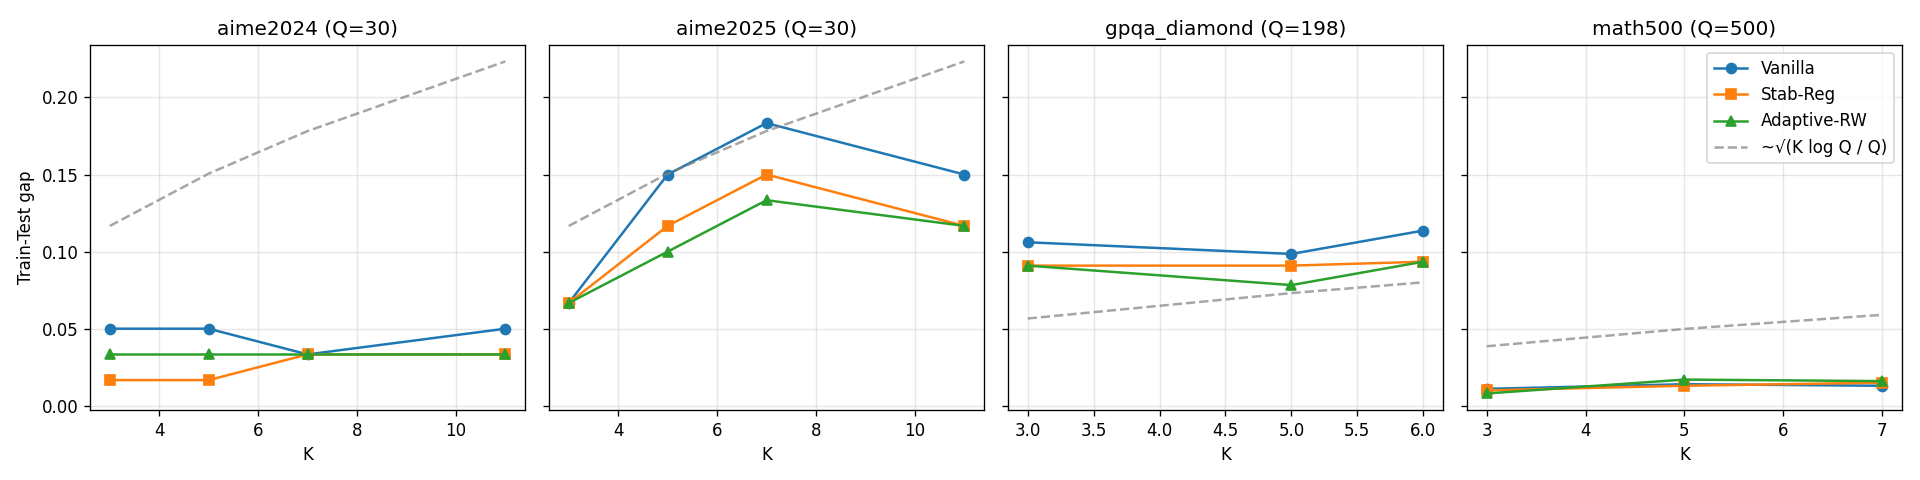
\includegraphics[width=0.49\linewidth]{buffered_figures/legacy_k_scaling.png}
\hfill
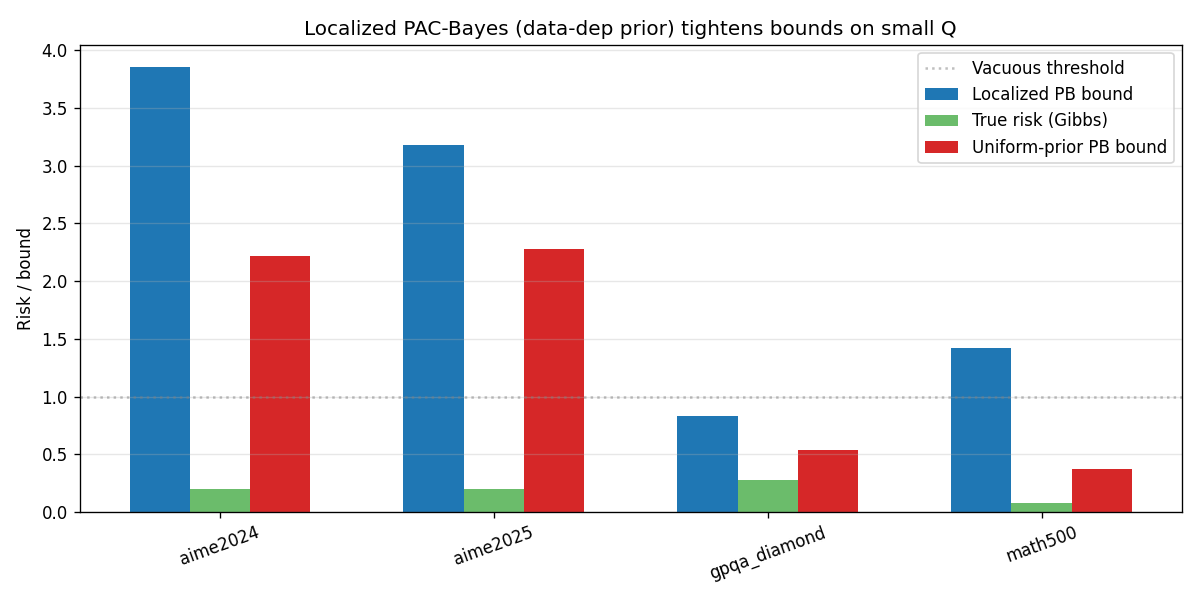
\includegraphics[width=0.49\linewidth]{buffered_figures/legacy_pac_bayes.png}
\caption{Additional retained diagnostics.  Left: dependence of measured gaps
on the number of ensemble members.  Right: localized and uniform-prior
PAC--Bayes values.  These are auxiliary diagnostics rather than evidence for
the buffered-ERM theorem.}
\label{fig:legacy-aux}
\end{figure}

\paragraph{Artifact record.}
The complete numerical object is
\path{zhi_code/src/working/experiment_data.json}; plots are in the same
directory.  The inputs are the tracked files under
\path{zhi_code/reference_data/jsonl}.  Appendix~\ref{app:legacy-full-data}
transcribes every field with completed numerical content in that object.  The
expanded synthetic tables in the earlier long appendix are omitted because no
matching saved artifacts were found.
